% Options for packages loaded elsewhere
\PassOptionsToPackage{unicode}{hyperref}
\PassOptionsToPackage{hyphens}{url}
%
\documentclass[
]{article}
\usepackage{amsmath,amssymb}
\usepackage{lmodern}
\usepackage{iftex}
\ifPDFTeX
  \usepackage[T1]{fontenc}
  \usepackage[utf8]{inputenc}
  \usepackage{textcomp} % provide euro and other symbols
\else % if luatex or xetex
  \usepackage{unicode-math}
  \defaultfontfeatures{Scale=MatchLowercase}
  \defaultfontfeatures[\rmfamily]{Ligatures=TeX,Scale=1}
\fi
% Use upquote if available, for straight quotes in verbatim environments
\IfFileExists{upquote.sty}{\usepackage{upquote}}{}
\IfFileExists{microtype.sty}{% use microtype if available
  \usepackage[]{microtype}
  \UseMicrotypeSet[protrusion]{basicmath} % disable protrusion for tt fonts
}{}
\makeatletter
\@ifundefined{KOMAClassName}{% if non-KOMA class
  \IfFileExists{parskip.sty}{%
    \usepackage{parskip}
  }{% else
    \setlength{\parindent}{0pt}
    \setlength{\parskip}{6pt plus 2pt minus 1pt}}
}{% if KOMA class
  \KOMAoptions{parskip=half}}
\makeatother
\usepackage{xcolor}
\IfFileExists{xurl.sty}{\usepackage{xurl}}{} % add URL line breaks if available
\IfFileExists{bookmark.sty}{\usepackage{bookmark}}{\usepackage{hyperref}}
\hypersetup{
  pdftitle={Codebook for survdf},
  hidelinks,
  pdfcreator={LaTeX via pandoc}}
\urlstyle{same} % disable monospaced font for URLs
\usepackage[margin=2cm]{geometry}
\usepackage{longtable,booktabs,array}
\usepackage{calc} % for calculating minipage widths
% Correct order of tables after \paragraph or \subparagraph
\usepackage{etoolbox}
\makeatletter
\patchcmd\longtable{\par}{\if@noskipsec\mbox{}\fi\par}{}{}
\makeatother
% Allow footnotes in longtable head/foot
\IfFileExists{footnotehyper.sty}{\usepackage{footnotehyper}}{\usepackage{footnote}}
\makesavenoteenv{longtable}
\usepackage{graphicx}
\makeatletter
\def\maxwidth{\ifdim\Gin@nat@width>\linewidth\linewidth\else\Gin@nat@width\fi}
\def\maxheight{\ifdim\Gin@nat@height>\textheight\textheight\else\Gin@nat@height\fi}
\makeatother
% Scale images if necessary, so that they will not overflow the page
% margins by default, and it is still possible to overwrite the defaults
% using explicit options in \includegraphics[width, height, ...]{}
\setkeys{Gin}{width=\maxwidth,height=\maxheight,keepaspectratio}
% Set default figure placement to htbp
\makeatletter
\def\fps@figure{htbp}
\makeatother
\setlength{\emergencystretch}{3em} % prevent overfull lines
\providecommand{\tightlist}{%
  \setlength{\itemsep}{0pt}\setlength{\parskip}{0pt}}
\setcounter{secnumdepth}{-\maxdimen} % remove section numbering
\newcommand{\fullline}{\noindent\makebox[\linewidth]{\rule{\textwidth}{0.4pt}}}
\renewcommand\familydefault{\sfdefault}
\newcommand{\bminione}{\begin{minipage}{0.75 \textwidth}}
\newcommand{\bminitwo}{\begin{minipage}{0.25 \textwidth}}
\newcommand{\emini}{\end{minipage}}
\ifLuaTeX
  \usepackage{selnolig}  % disable illegal ligatures
\fi

\title{Codebook for survdf}
\usepackage{etoolbox}
\makeatletter
\providecommand{\subtitle}[1]{% add subtitle to \maketitle
  \apptocmd{\@title}{\par {\large #1 \par}}{}{}
}
\makeatother
\subtitle{Autogenerated data summary from dataMaid}
\author{}
\date{\vspace{-2.5em}2022-06-10 19:37:02}

\begin{document}
\maketitle

\hypertarget{data-report-overview}{%
\section{Data report overview}\label{data-report-overview}}

The dataset examined has the following dimensions:

\begin{longtable}[]{@{}
  >{\raggedright\arraybackslash}p{(\columnwidth - 2\tabcolsep) * \real{0.3472}}
  >{\raggedleft\arraybackslash}p{(\columnwidth - 2\tabcolsep) * \real{0.1250}}@{}}
\toprule
\begin{minipage}[b]{\linewidth}\raggedright
Feature
\end{minipage} & \begin{minipage}[b]{\linewidth}\raggedleft
Result
\end{minipage} \\
\midrule
\endhead
Number of observations & 20 \\
Number of variables & 3 \\
\bottomrule
\end{longtable}

\hypertarget{codebook-summary-table}{%
\section{Codebook summary table}\label{codebook-summary-table}}

\begin{longtable}[]{@{}
  >{\raggedright\arraybackslash}p{(\columnwidth - 10\tabcolsep) * \real{0.1923}}
  >{\raggedright\arraybackslash}p{(\columnwidth - 10\tabcolsep) * \real{0.2308}}
  >{\raggedright\arraybackslash}p{(\columnwidth - 10\tabcolsep) * \real{0.1282}}
  >{\raggedleft\arraybackslash}p{(\columnwidth - 10\tabcolsep) * \real{0.1410}}
  >{\centering\arraybackslash}p{(\columnwidth - 10\tabcolsep) * \real{0.1282}}
  >{\raggedright\arraybackslash}p{(\columnwidth - 10\tabcolsep) * \real{0.1795}}@{}}
\toprule
\begin{minipage}[b]{\linewidth}\raggedright
Label
\end{minipage} & \begin{minipage}[b]{\linewidth}\raggedright
Variable
\end{minipage} & \begin{minipage}[b]{\linewidth}\raggedright
Class
\end{minipage} & \begin{minipage}[b]{\linewidth}\raggedleft
\# unique values
\end{minipage} & \begin{minipage}[b]{\linewidth}\centering
Missing
\end{minipage} & \begin{minipage}[b]{\linewidth}\raggedright
Description
\end{minipage} \\
\midrule
\endhead
low dosage (4.5 micromols per square meter per second), medium dosage
(6.75 micromols per square meter per second), high dosage (9 micromols
per square meter per second) & \textbf{\protect\hyperlink{light}{Light}}
& factor & 3 & 0.00 \% & \\
low dosage (2 NTUs), medium dosage (5.5 NTUs), high dosage (9 NTUs) &
\textbf{\protect\hyperlink{turbidity}{Turbidity}} & factor & 3 & 0.00 \%
& \\
Percentage of early-stage Delta smelt larvae (0-40 days post hatch) that
survived & \textbf{\protect\hyperlink{survival}{Survival}} & numeric &
20 & 0.00 \% & \\
\bottomrule
\end{longtable}

\hypertarget{variable-list}{%
\section{Variable list}\label{variable-list}}

\hypertarget{light}{%
\subsection{Light}\label{light}}

\emph{low dosage (4.5 micromols per square meter per second), medium
dosage (6.75 micromols per square meter per second), high dosage (9
micromols per square meter per second)}

\begin{minipage}{0.75 \textwidth}

\begin{longtable}[]{@{}
  >{\raggedright\arraybackslash}p{(\columnwidth - 2\tabcolsep) * \real{0.3611}}
  >{\raggedleft\arraybackslash}p{(\columnwidth - 2\tabcolsep) * \real{0.1389}}@{}}
\toprule
\begin{minipage}[b]{\linewidth}\raggedright
Feature
\end{minipage} & \begin{minipage}[b]{\linewidth}\raggedleft
Result
\end{minipage} \\
\midrule
\endhead
Variable type & factor \\
Number of missing obs. & 0 (0 \%) \\
Number of unique values & 3 \\
Mode & ``low'' \\
Reference category & low \\
\bottomrule
\end{longtable}

\end{minipage}
\begin{minipage}{0.25 \textwidth}

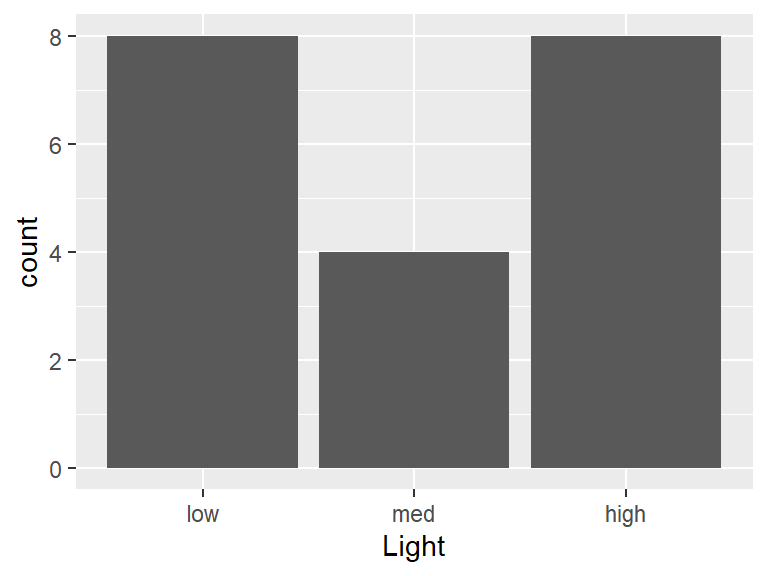
\includegraphics{codebook_survdf_files/figure-latex/Var-1-Light-1.pdf}

\end{minipage}

\begin{itemize}
\tightlist
\item
  Observed factor levels: "high", "low", "med".
\end{itemize}

\noindent\makebox[\linewidth]{\rule{\textwidth}{0.4pt}}

\hypertarget{turbidity}{%
\subsection{Turbidity}\label{turbidity}}

\emph{low dosage (2 NTUs), medium dosage (5.5 NTUs), high dosage (9
NTUs)}

\begin{minipage}{0.75 \textwidth}

\begin{longtable}[]{@{}
  >{\raggedright\arraybackslash}p{(\columnwidth - 2\tabcolsep) * \real{0.3611}}
  >{\raggedleft\arraybackslash}p{(\columnwidth - 2\tabcolsep) * \real{0.1389}}@{}}
\toprule
\begin{minipage}[b]{\linewidth}\raggedright
Feature
\end{minipage} & \begin{minipage}[b]{\linewidth}\raggedleft
Result
\end{minipage} \\
\midrule
\endhead
Variable type & factor \\
Number of missing obs. & 0 (0 \%) \\
Number of unique values & 3 \\
Mode & ``low'' \\
Reference category & low \\
\bottomrule
\end{longtable}

\end{minipage}
\begin{minipage}{0.25 \textwidth}

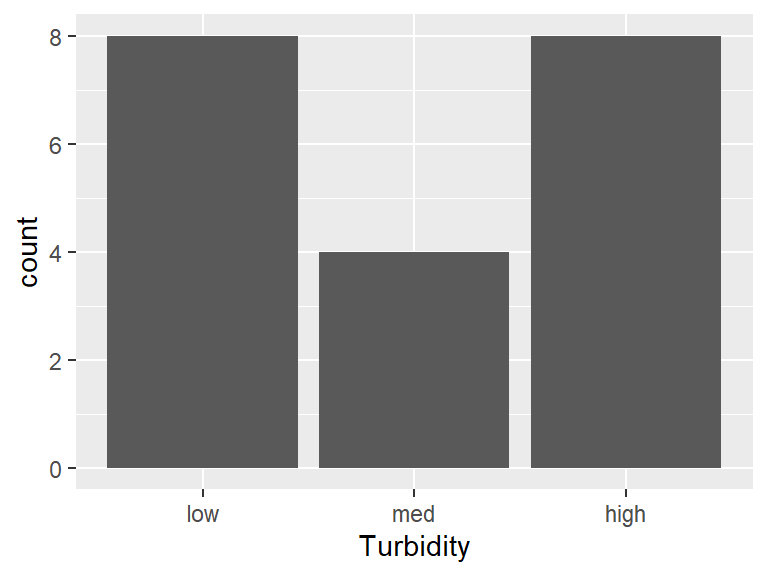
\includegraphics{codebook_survdf_files/figure-latex/Var-2-Turbidity-1.pdf}

\end{minipage}

\begin{itemize}
\tightlist
\item
  Observed factor levels: "high", "low", "med".
\end{itemize}

\noindent\makebox[\linewidth]{\rule{\textwidth}{0.4pt}}

\hypertarget{survival}{%
\subsection{Survival}\label{survival}}

\emph{Percentage of early-stage Delta smelt larvae (0-40 days post
hatch) that survived}

\begin{minipage}{0.75 \textwidth}

\begin{longtable}[]{@{}
  >{\raggedright\arraybackslash}p{(\columnwidth - 2\tabcolsep) * \real{0.3611}}
  >{\raggedleft\arraybackslash}p{(\columnwidth - 2\tabcolsep) * \real{0.2083}}@{}}
\toprule
\begin{minipage}[b]{\linewidth}\raggedright
Feature
\end{minipage} & \begin{minipage}[b]{\linewidth}\raggedleft
Result
\end{minipage} \\
\midrule
\endhead
Variable type & numeric \\
Number of missing obs. & 0 (0 \%) \\
Number of unique values & 20 \\
Median & 59.56 \\
1st and 3rd quartiles & 55.79; 67.24 \\
Min. and max. & 45.02; 89.09 \\
\bottomrule
\end{longtable}

\end{minipage}
\begin{minipage}{0.25 \textwidth}

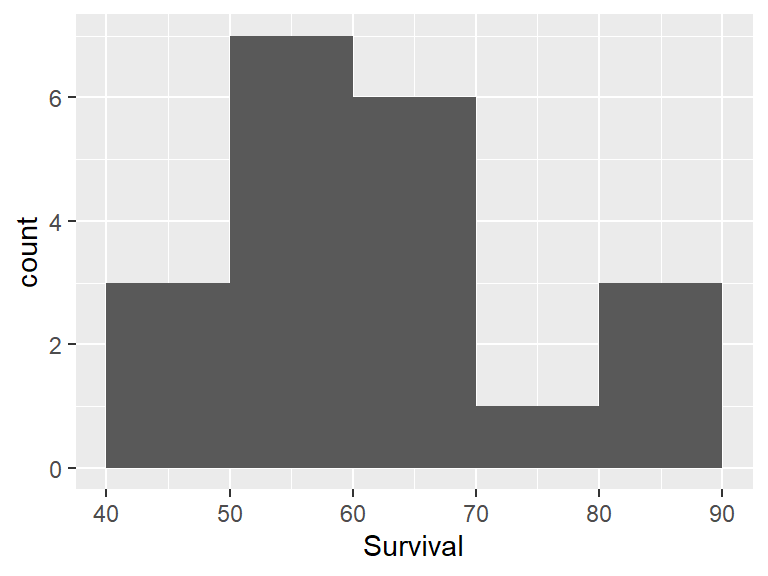
\includegraphics{codebook_survdf_files/figure-latex/Var-3-Survival-1.pdf}

\end{minipage}

\noindent\makebox[\linewidth]{\rule{\textwidth}{0.4pt}}

Report generation information:

\begin{itemize}
\item
  Created by: emontoya2 (username: \texttt{monto}).
\item
  Report creation time: Fri Jun 10 2022 19:37:03
\item
  Report was run from directory:
  \texttt{C:/Users/monto/Desktop/gprojects/tmsm/tmsm}
\item
  dataMaid v1.4.1 {[}Pkg: 2021-10-08 from CRAN (R 4.1.3){]}
\item
  R version 4.1.2 (2021-11-01).
\item
  Platform: x86\_64-w64-mingw32/x64 (64-bit)(Windows 10 x64 (build
  22000)).
\item
  Function call:
  \texttt{dataMaid::makeDataReport(data\ =\ survdf,\ mode\ =\ c("summarize",\ \ "visualize",\ "check"),\ smartNum\ =\ FALSE,\ file\ =\ "codebook\_survdf.Rmd",\ \ \ \ \ \ checks\ =\ list(character\ =\ "showAllFactorLevels",\ factor\ =\ "showAllFactorLevels",\ \ \ \ \ \ \ \ \ \ labelled\ =\ "showAllFactorLevels",\ haven\_labelled\ =\ "showAllFactorLevels",\ \ \ \ \ \ \ \ \ \ numeric\ =\ NULL,\ integer\ =\ NULL,\ logical\ =\ NULL,\ Date\ =\ NULL),\ \ \ \ \ \ listChecks\ =\ FALSE,\ maxProbVals\ =\ Inf,\ codebook\ =\ TRUE,\ reportTitle\ =\ "Codebook\ for\ survdf")}
\end{itemize}

\end{document}
